%---------------------------------------------------------------
\chapter{Misspecified models experiments}
\label{chap:misspecified}
%---------------------------------------------------------------

The purpose of this chapter is to illustrate how the tracking performance of the filters will change if the noise of the measurement model is misspecified or even unknown. The main question and interest is how much better the ABC filters will show themselves under these conditions compared to the others. It is important to remember that the ABC filters ignore the properties of measurement noise, which make them suitable for use directly in such situations, as opposed to the standard PF or KF (or its extended version), where modifications are usually required without much guarantee of success unless laborious tuning is done.

To keep the experiments honest, the same models as in the previous chapter will be used, with the same structure, except that the measurement noise will be Cauchy distributed. At the same time, it will be interesting to see the results of tracking KF and its extended version since they require both state and measurement noises te be Gaussian for optimality. If the first condition remains, the measurement noise in this chapter will use Cauchy distributed, which should already complicate the tracking performance of KFs. KF is expected to work normally for most noise distributions as long as the errors have a zero mean and the distributions are symmetric around the mean. But it will no longer be optimal under Cauchy noise conditions.

The metric for measuring performance in this chapter will remain the same, that is, MSE will be used. The same filters as in the previous chapter will take part in the experiments: the PF, ABC filters with normal and Cauchy kernels, as well as the Kalman filter for linear models and its extended version for nonlinear models.

\section{Example 1: Power growth model}
It is the turn to return to the model described in detail in the last chapter, namely, the PGM, which is characterized by the equations (\ref{eq:pgm_equations}). As previously stated, the constructed SSM remains the same as the initialization parameters of the filters. Since dealing with the misspecified model in this chapter, the same measurement model (\ref{eq:pgm_measurement_model}) is used, but this time all measurements are corrupted by Cauchy noise instead of Gaussian, keeping the scaling parameter equal to 10:

\begin{equation}
\begin{aligned}
\varepsilon_t \sim \mathcal{C}\text{auchy}\left(0, 10^2\right)
\end{aligned}
\end{equation}

As before,  an experiment with 100 repetitions was conducted to obtain representative results. At this point it can be moved directly to the analysis of the results of the experiment itself.

\paragraph*{Charts and analysis} 
The analysis will begin again with the MSE values, shown in Figure \ref{fig:pgm_mse_boxplot_cauchy} and Table \ref{table:pgm_mse_cauchy}, where the Figure shows the statistics of the final MSE values of 100 repeated experiment runs and the Table accordingly shows their averaged values. As one can immediately notice, there are no MSE values for the EKF filter because it failed to cope with tracking in any of the experiment runs. Already in the initial stages of filtering, the EKF led to invalid values. The filters of the SMC family avoided this by modifying the particle evolution function discussed in the previous chapter. As already mentioned in the previous chapter, in the context of this model, it can be noted that the choice of the kernel has no noticeable effect on the tracking performance of the ABC filters.

As for the MSE values, when one looks at the box plots and the Table with averaged values, the superiority of ABC filters over the PF filter becomes immediately apparent, especially with respect to tracking the variable \(x_1\). It is noticeable that in some experiment runs, the final MSE values of both ABC filters were critically high, but according to the averaged values, which are relatively low, one can conclude that, in general, both filters were quite stable under heavy-tailed noise. That can not be said about the PF filter, which failed to track the variable \(x_1\).

\begin{figure}[!ht]
\centering
\caption{(PGM, Cauchy noise) Box plots showing final MSE values for both state variables \(\mu\) and \(\nu\) of 100 repeated experiments. The boxes show medians, upper and lower quartiles. The length of the whiskers is defined as 1.5 times the interquartile range. The outliers are not displayed.}
\subfloat{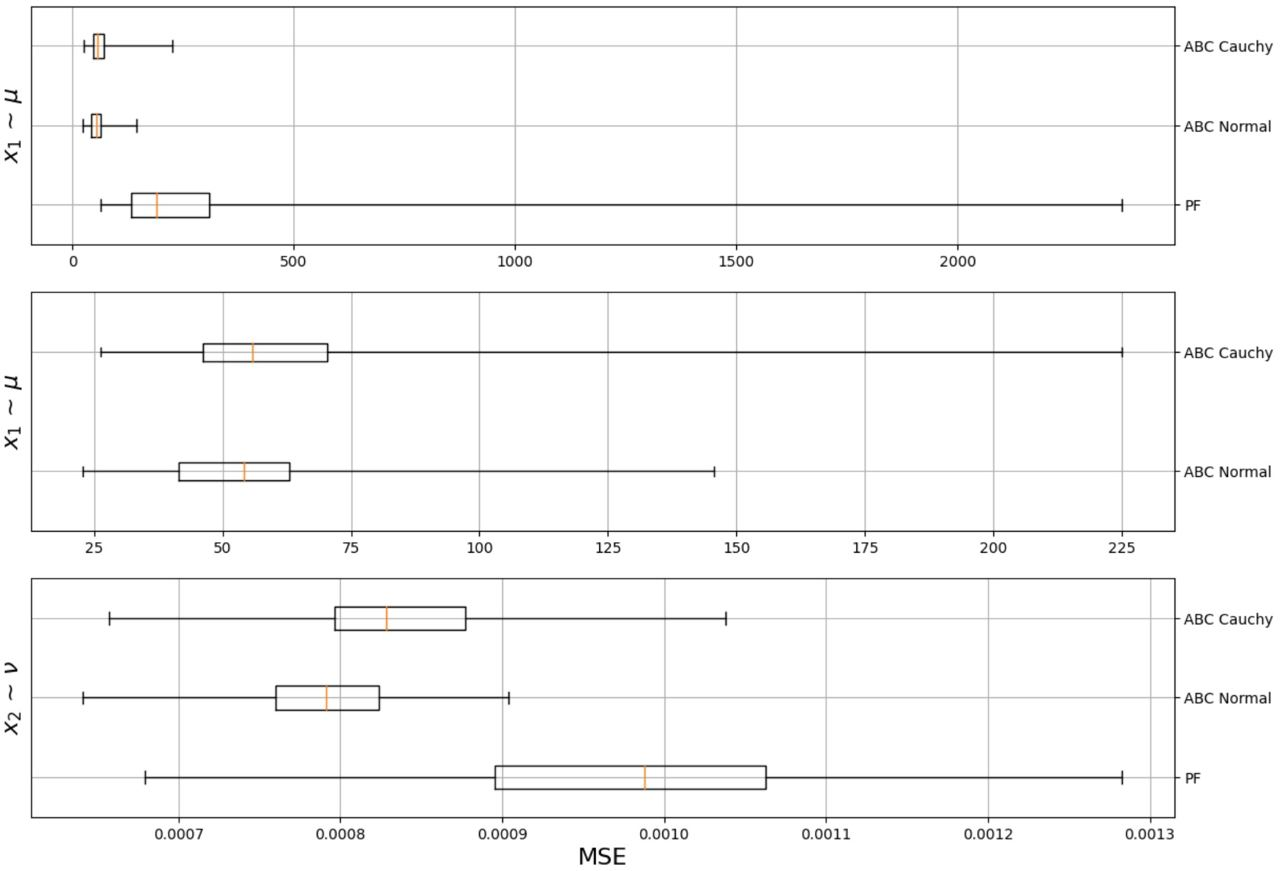
\includegraphics[width=0.9\columnwidth, height=\textheight,keepaspectratio]{figures/pgm/mse_boxplot_cauchy.jpg}}
\label{fig:pgm_mse_boxplot_cauchy}
\end{figure}

\begin{table}[h!]
\centering
\begin{tabular}{ |p{4cm}|p{4cm}|p{4cm}|}
 \hline 
  & \(\mu\) & \(\nu\)\\
 \hline \hline
 EKF & - & - \\
 PF & 271.668  & 9.830e-04 \\
 ABC Normal & 56.660 & 7.899e-04\\
 ABC Cauchy & 64.265 & 8.366e-04\\
 \hline
\end{tabular}
\caption{(PGM, Cauchy noise) The final MSE values for both state variables \(\mu\) and \(\nu\) averaged over 100 runs}
\label{table:pgm_mse_cauchy}
\end{table}

Figure \ref{fig:pgm_measurement_noise_cauchy} shows a noise realization from one of the 100 experiments. A noise time series for a single experiment run is shown in Figure \ref{fig:pgm_abc_scales_evolution_cauchy}, along with evolutions of the normal and Cauchy kernel scales. From the example of this data, it is well seen that both ABC filters reflect well the noise evolution, regardless of the choice of kernel.

\begin{figure}[!ht]
\centering
\caption{(PGM, Cauchy noise) One particular Cauchy noise realization \(\varepsilon_t\). Relative frequency histogram limited to [-120; 120] and scale-broken box plot. The box plot consists of three parts. The central part is a box that includes the median, upper and lower quartiles. The length of the whiskers is defined as 1.5 times the interquartile range. Outliers and extreme values are displayed on the left and right, respectively.}
\subfloat{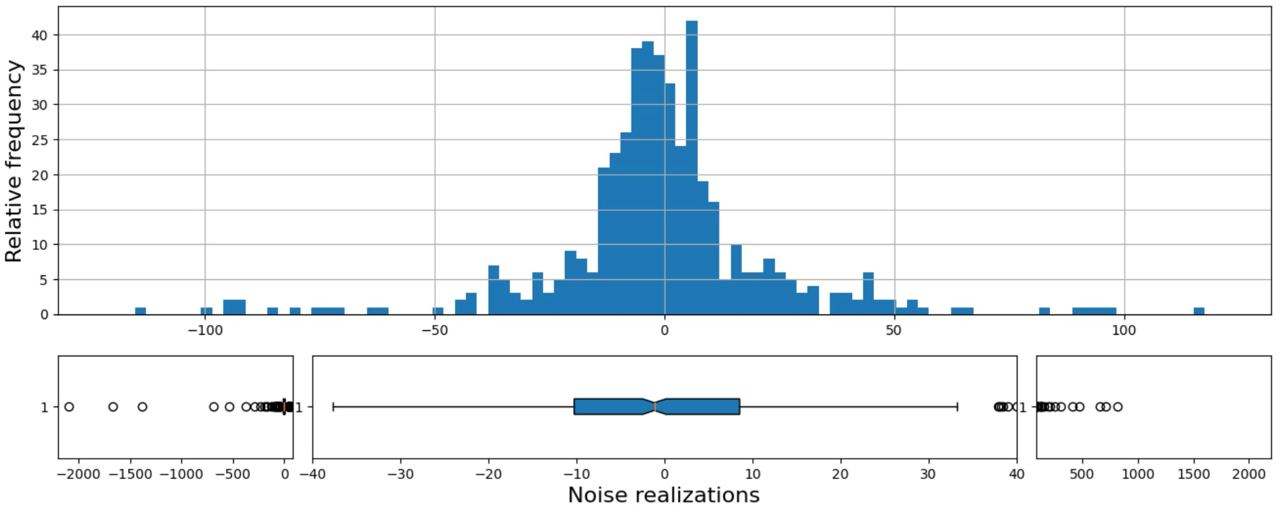
\includegraphics[width=0.9\columnwidth, height=\textheight,keepaspectratio]{figures/pgm/measurement_noise_cauchy.jpg}}
\label{fig:pgm_measurement_noise_cauchy}
\end{figure}

\begin{figure}[!ht]
\centering
\caption{(PGM, Cauchy noise) The top two graphs show the one particular evolution of the normal and Cauchy scales \(\varepsilon_t\), respectively. The lower one represents the Cauchy noise realizations.}
\subfloat{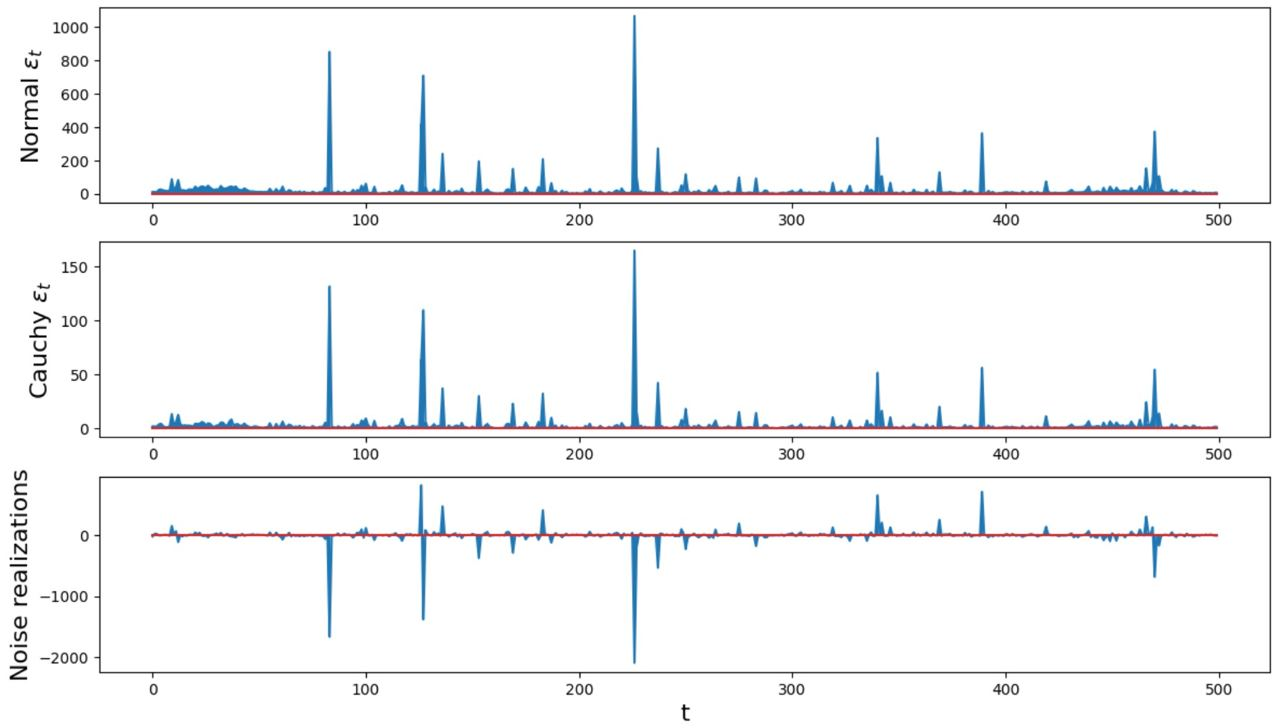
\includegraphics[width=0.9\columnwidth, height=\textheight,keepaspectratio]{figures/pgm/abc_scales_evolution_cauchy.jpg}}
\label{fig:pgm_abc_scales_evolution_cauchy}
\end{figure}

\section{Example 2: Constant velocity model}
In this section, the discussion will focus on the model already described earlier, namely the CVM. The model itself is characterized by the following equations (\ref{eq:cvm_equations}) and (\ref{eq:cvm_measurement_equation}). As mentioned earlier, the initialization parameters of the filters are not changed the same way as the constructed SSM. Also, the same measurement model is used (\ref{eq:cvm_measurement_model}), but all measurements in this example are corrupted by Cauchy distributed noise instead of Gaussian, keeping the same scaling parameter:

\begin{equation}
\begin{aligned}
\varepsilon_t \sim \mathcal{C}\text{auchy}\left(0, R_t\right) \quad \text{with} \quad R =
    3^{2}\cdot
    \begin{bmatrix}
        1 & 0 \\
        0 & 1
    \end{bmatrix}
\end{aligned}
\end{equation}

In order to obtain representative results, an experiment with 100 repetitions was conducted. 

\paragraph*{Charts and analysis}
Following the already usual approach, the analysis will focus on the MSE values, which can be found in Figure \ref{fig:cvm_mse_boxplot_cauchy} representing the statistic of the final MSE values of 100 repeated experiment runs, and in Table \ref{table:cvm_mse_cauchy}, which shows their averaged values.

Again it can be noted that, in general, the ABC filters showed the best results among the other filters, in the predominant number of repetitions of the experiment had the minimum final MSE, which is also well reflected in the Table of averaged values. The ABC filter in the normal kernel was closer to the true values when tracing, which can be seen in all box plots, and as a consequence, it has lower values of the averaged MSE for all state variables compared to the ABC filter with the Cauchy kernel. But on the whole, the ABC filter with the Cauchy kernel also showed decent results in the prevailing number of runs of the experiment.

As for the PF filter, it can be safely said that it had enough trouble tracking all state variables, which is reflected in its MSE values. If in the context of this experiment, ABC filters with both kernels showed themselves as relatively stable under heavy-tailed noise, the same cannot be said about the PF filter.

Regarding the KF filter and box plots of its final MSE values, it can be stated that in the majority of cases, the filter was quite accurate in tracking, but judging by the maximum final MSE values, which are very far from the medians on all box plots, one can judge that in some rare runs the filter absolutely failed. That also confirms the statement about its non-optimality under the given conditions. The consequence of the maximum MSE values is also displayed on the averaged MSE values in the Table \ref{table:cvm_mse_cauchy}.

\begin{figure}[!ht]
\centering
\caption{(CVM, Cauchy noise)  Box plots showing final MSE values for all state variables $x_1$, $x_2$, $v_1$ and $v_2$ of 100 repeated experiments. The boxes show medians, upper and lower quartiles. The length of the whiskers is defined as 1.5 times the interquartile range. The outliers are not displayed.}
\subfloat{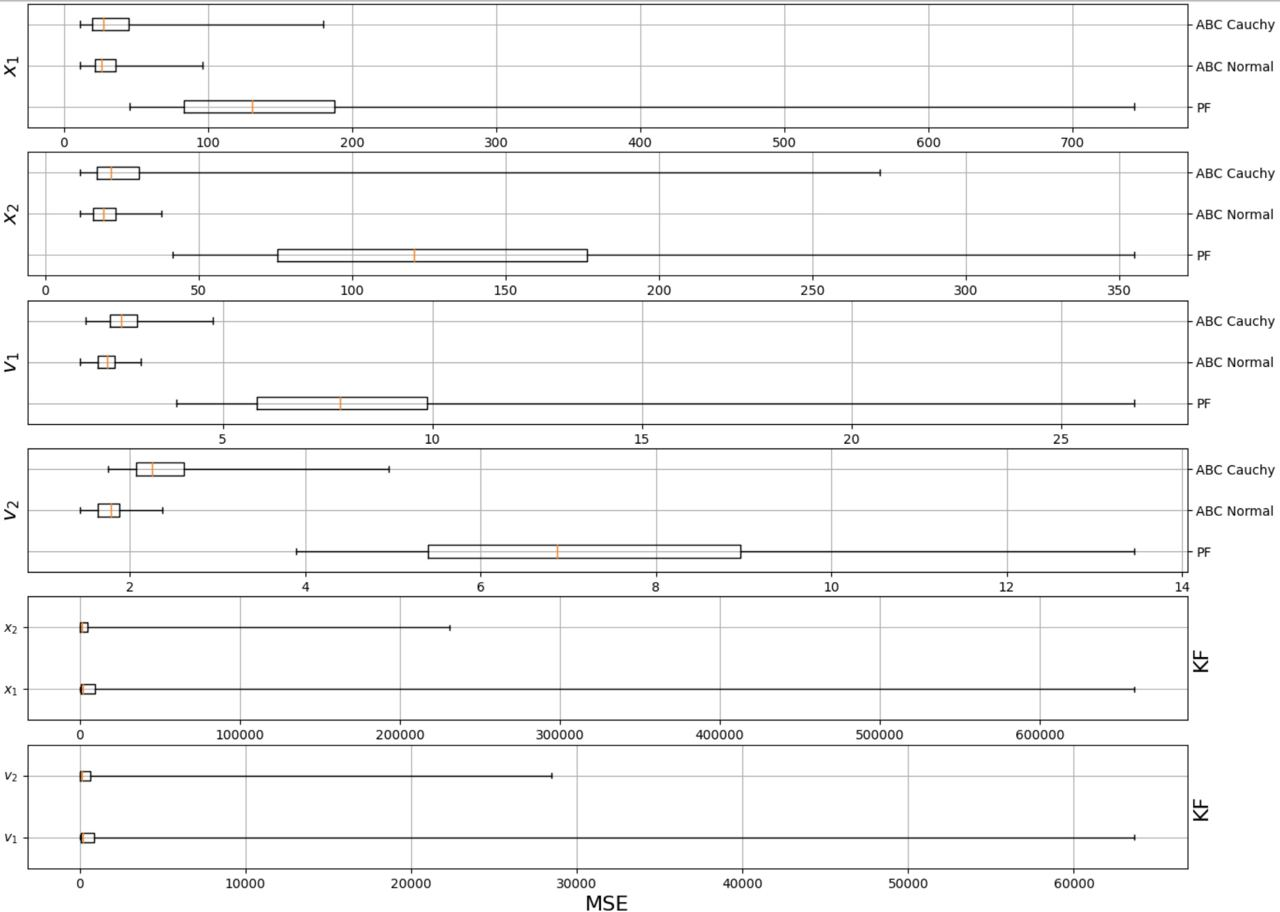
\includegraphics[width=0.9\columnwidth, height=\textheight,keepaspectratio]{figures/cvm/mse_boxplot_cauchy.jpg}}
\label{fig:cvm_mse_boxplot_cauchy}
\end{figure}

\begin{table}[h!]
\centering
\begin{tabular}{ |p{2cm}|p{2cm}|p{2cm}|p{2cm}|p{2cm}|}
 \hline 
  & $x_1$ & $x_2$ & $v_1$ & $v_2$ \\
 \hline \hline
 KF & 303.669e+03 & 268.659e+07 & 294.374e+02 & 259.620e+06  \\
 PF & 162.614 & 129.882 & 8.701 & 7.302 \\
 ABC Normal & 29.952 & 19.894 & 2.244 & 1.781 \\
 ABC Cauchy & 38.065 & 29.674 & 2.721 & 2.390 \\
 \hline
\end{tabular}
\caption{(CVM, Cauchy noise) The final MSE values for all state variables $x_1$, $x_2$, $v_1$ and $v_2$ averaged over 100 runs}
\label{table:cvm_mse_cauchy}
\end{table}


Again, to evaluate the effectiveness of ABC filters, it is worth looking at Figure \ref{fig:cvm_measurement_noise_cauchy}, which shows a noise realization from one of the 100 experiments, and also, at  Figure \ref{fig:cvm_abc_scales_evolution_cauchy} which shows a noise time series for a single experiment run, along with evolutions of the normal and Cauchy kernel scales. It is clear that both ABC filters reflect well the noise evolution, even the significant values.

\begin{figure}[!ht]
\centering
\caption{(CVM, Cauchy noise) One particular Cauchy noise realizations \(\varepsilon_{y_1,t}\) and \(\varepsilon_{y_2,t}\). Relative frequency histograms limited to [-60; 60] and scale-broken box plots. Each box plot consists of three parts. The central part is a box that includes the median, upper and lower quartiles. The length of the whiskers is defined as 1.5 times the interquartile range. Outliers and extreme values are displayed on the left and right, respectively.}
\subfloat{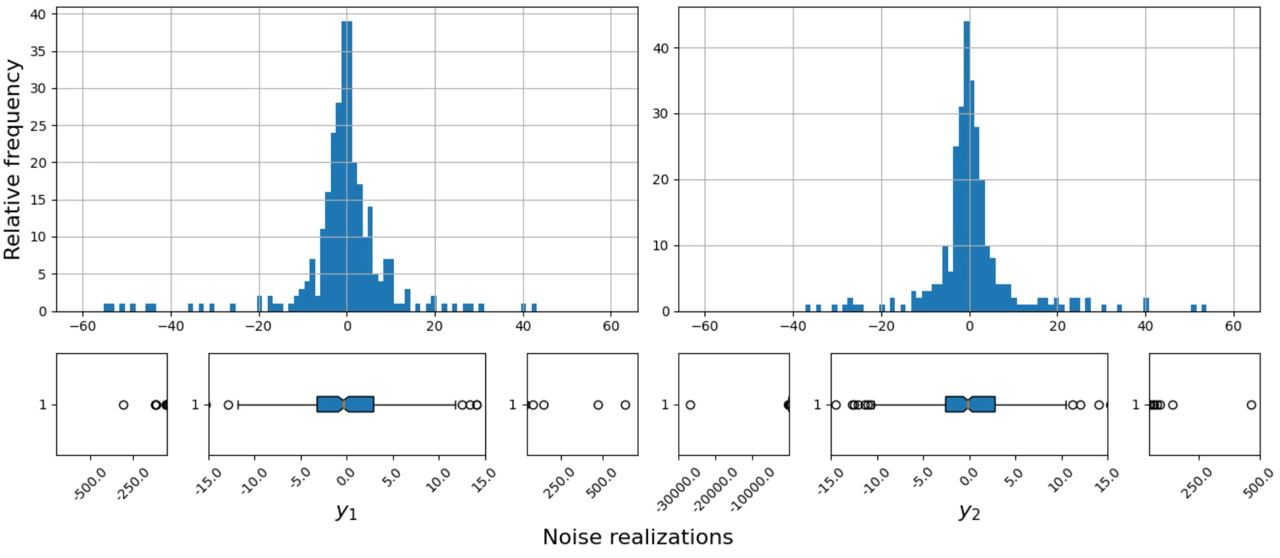
\includegraphics[width=0.9\columnwidth, height=\textheight,keepaspectratio]{figures/cvm/measurement_noise_cauchy.jpg}}
\label{fig:cvm_measurement_noise_cauchy}
\end{figure}

\begin{figure}[!ht]
\centering
\caption{(CVM, Cauchy noise) The top four graphs show the one particular evolution of the normal and Cauchy scales \(\varepsilon_{y_1,t}, \varepsilon_{y_2,t}\), respectively. The bottom two represent the Cauchy noise realizations.}
\subfloat{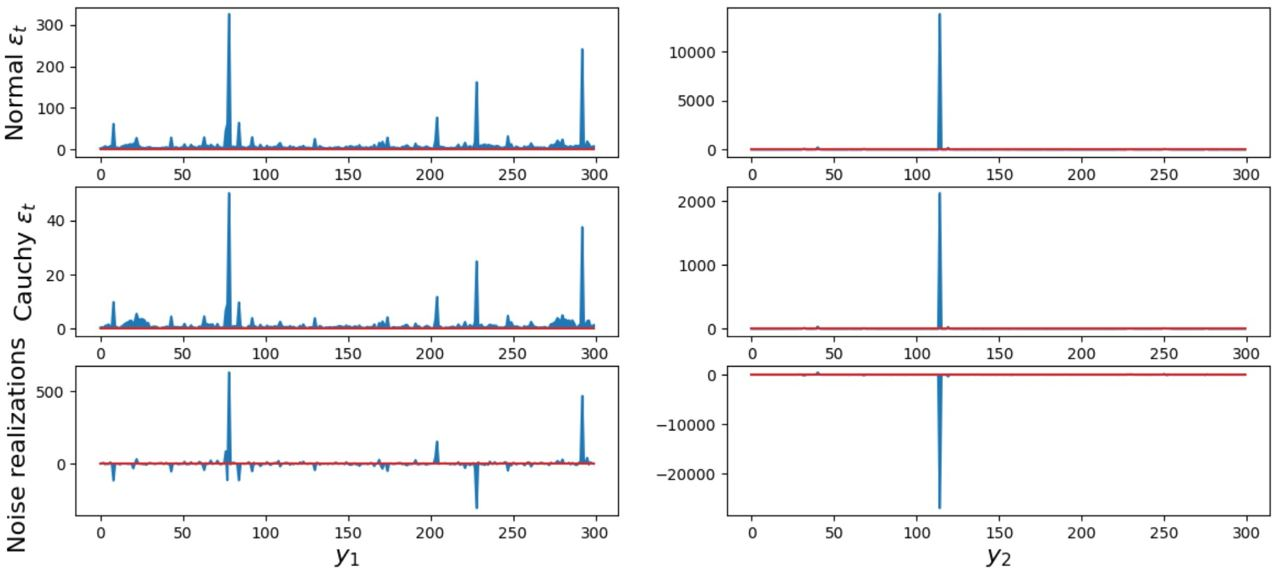
\includegraphics[width=0.9\columnwidth, height=\textheight,keepaspectratio]{figures/cvm/abc_scales_evolution_cauchy.jpg}}
\label{fig:cvm_abc_scales_evolution_cauchy}
\end{figure}

\section{Example 3: Polar radar model}
Returning to the PRM, which is described by the following equations (\ref{eq:cvm_equations}) and (\ref{eq:prm_equations}), leaving everything unchanged for the honesty of the experiment, except that all measurements will be corrupted by Cauchy distributed noise. In addition, the initialization parameters of the filters are not changed. The same noise scale parameter remains. The measurement noise is as follows:

\begin{equation}
    \varepsilon_t \sim \mathcal{C}\text{auchy}\left(0, R_t\right) \quad \text{with} \quad R =
    3^{2}\cdot
    \begin{bmatrix}
        0.01 & 0.0 & 0.0 \\
        0.0 & 0.0001 & 0.0 \\
        0.0 & 0.0 & 0.01
    \end{bmatrix}.
\end{equation}

In order to obtain representative results, an experiment with 100 repetitions was conducted.

\paragraph*{Charts and analysis}
As can be expected that the analysis will focus on the MSE values, which can be found in Figure \ref{fig:prm_mse_boxplot_cauchy}, which shows the statistics of the final MSE values of 100 repeated experiment runs, and in Table \ref{table:prm_mse_cauchy}, which contains their averaged values.

One can observe approximately the same situation as in the previous expert. But this time, both ABC filters really showed outstanding results. Minimal averaged MSE values in Table \ref{table:prm_mse_cauchy} show high robustness to different heavy noise realizations. It is worth noting that in the context of this experiment, the ABC filter with the Cauchy kernel performed slightly but better than the same filter with the normal kernel and generally has lower MSE values. It is also worth noting that the choice of the kernel has no significant impact on the effectiveness of the ABC filter.

As for the PF filter, the tendency for it to be inferior to ABC filters in this chapter continues, which is logical since it assumes a misspecified measurement model with normal noise. In general, it always has a much larger final MSE value, and at times, judging by the maximum values from the box plots, they are even critically significant. This is also reflected in the averaged values in the table \ref{table:prm_mse_cauchy}, especially for the state variables \(x_1\) and \(x_2\).

The last thing that has not been analyzed is the tracking efficiency of the EKF filter. It can be definitely said that the EKF filter suffered the same fate as the KF filter in the previous section within the CVM experiments.
That is, the prevailing number of runs EKF was quite close to the true values in its estimation process, but judging by the maximum values from the box plots, in rare cases, the final MSE values were critically high, which also affected the averaged MSE values in the Table \ref{table:prm_mse_cauchy}. That also confirms and indicates that the EKF filter is quite unstable under some heavy-tailed noise realizations.

\begin{figure}[!ht]
\centering
\caption{(PRM, Cauchy noise) Box plots showing final MSE values for all state variables $x_1$, $x_2$, $v_1$ and $v_2$ of 100 repeated experiments. The boxes show medians, upper and lower quartiles. The length of the whiskers is defined as 1.5 times the interquartile range. The outliers are not displayed.}
\subfloat{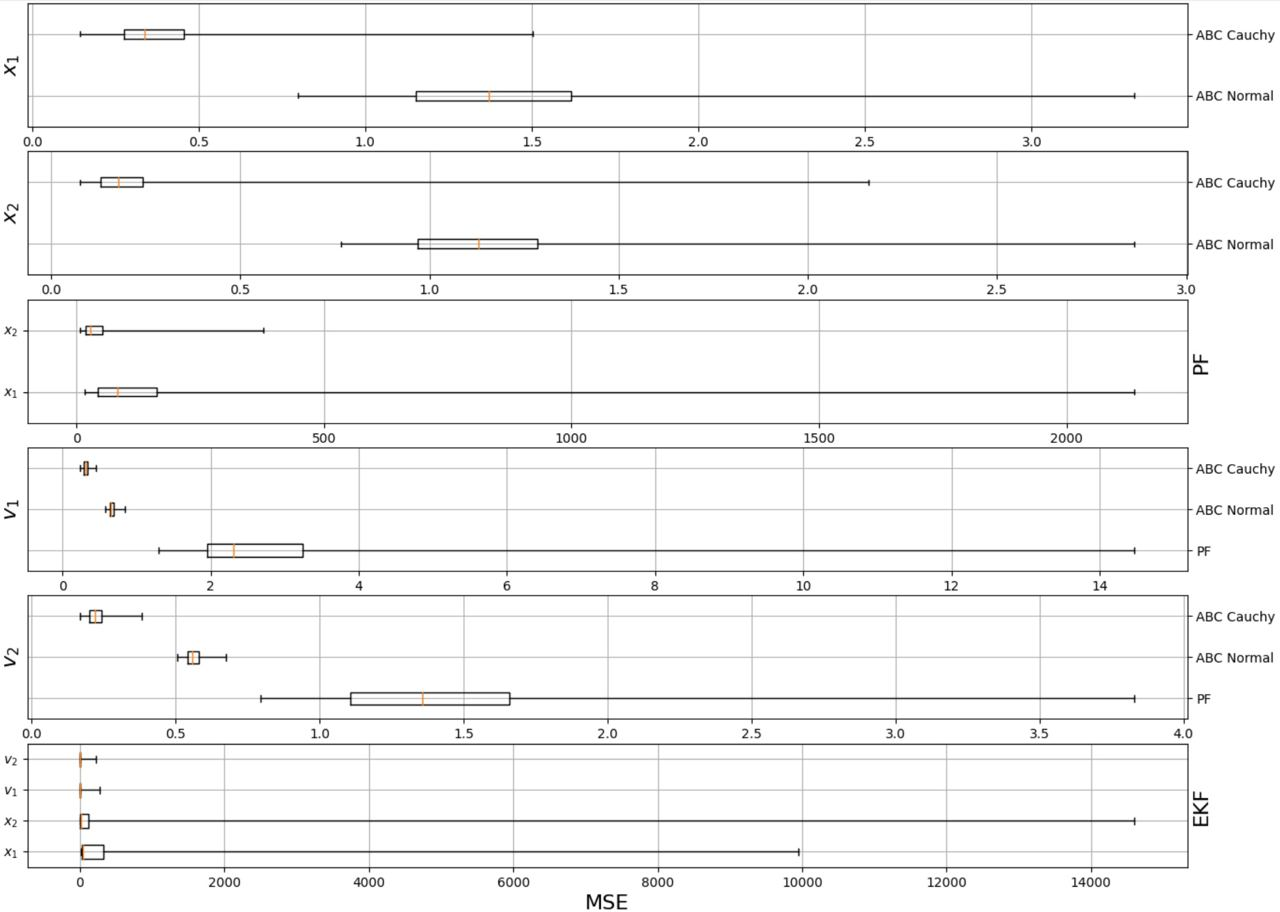
\includegraphics[width=0.9\columnwidth, height=\textheight,keepaspectratio]{figures/prm/mse_boxplot_cauchy.jpg}}
\label{fig:prm_mse_boxplot_cauchy}
\end{figure}

\begin{table}[h!]
\centering
\begin{tabular}{ |p{2cm}|p{2cm}|p{2cm}|p{2cm}|p{2cm}|}
 \hline 
  & $x_1$ & $x_2$ & $v_1$ & $v_2$ \\
 \hline \hline
 EKF & 620.381 & 466.478 & 15.570 & 10.575  \\
 PF & 184.171  & 48.923 & 3.017 & 1.484 \\
 ABC Normal & 1.450 & 1.182 & 0.664 & 0.562 \\
 ABC Cauchy & 0.401 & 0.222 & 0.316 & 0.227 \\
 \hline
\end{tabular}
\caption{(PRM, Cauchy noise) The final MSE values for all state variables $x_1$, $x_2$, $v_1$ and $v_2$ averaged over 100 runs}
\label{table:prm_mse_cauchy}
\end{table}

The Figure \ref{fig:prm_measurement_noise_cauchy} shows a noise realization from one of the 100 experiments. To evaluate how well the ABC filter with different kernels reflects the noise evolution is enough to look at Figure \ref{fig:cvm_abc_scales_evolution_cauchy}, which shows a noise time series for a single experiment run, along with evolutions of the normal and Cauchy kernel scales. It is absolutely clear that the ABC filter with both kernels captures noise evolution well.

\begin{figure}[!ht]
\centering
\caption{(PRM, Cauchy noise) One particular normal noise realizations \(\varepsilon_{y_1,t}\), \(\varepsilon_{y_2,t}\) and \(\varepsilon_{y_3,t}\). Relative frequency histograms and scale-broken box plots. The histograms on the sides are limited to [-0.4,0.4], and the middle one is limited to [-0.004,0.004]. Each box plot consists of three parts. The central part is a box that includes the median, upper and lower quartiles. The length of the whiskers is defined as 1.5 times the interquartile range. Outliers and extreme values are displayed on the left and right, respectively.}
\subfloat{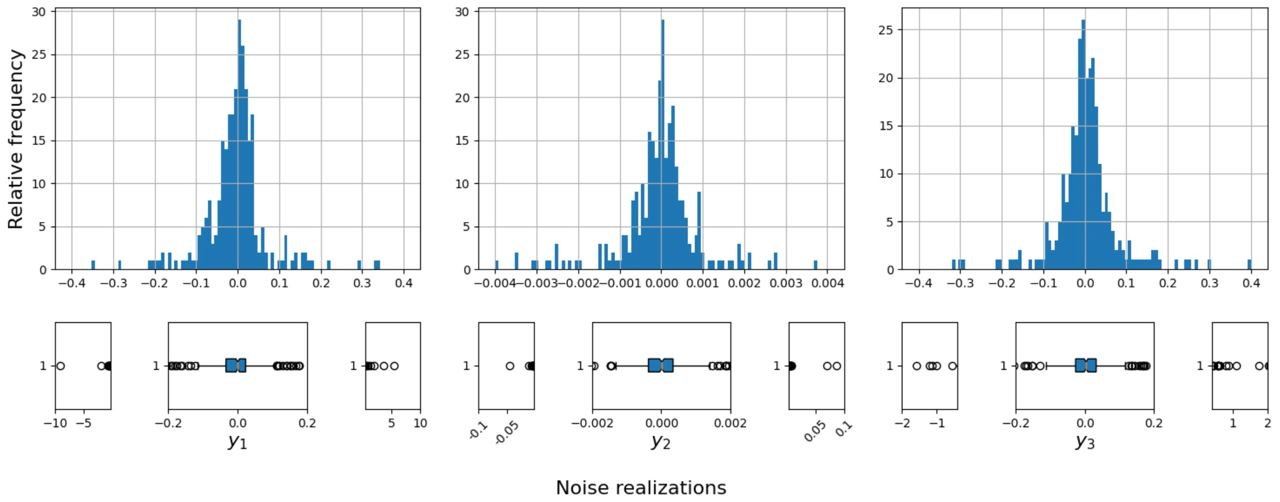
\includegraphics[width=0.9\columnwidth, height=\textheight,keepaspectratio]{figures/prm/measurement_noise_cauchy.jpg}}
\label{fig:prm_measurement_noise_cauchy}
\end{figure}

\begin{figure}[!ht]
\centering
\caption{(PRM, Cauchy noise) The top four graphs show the one particular evolution of the normal and Cauchy scales \(\varepsilon_{y_1,t}, \varepsilon_{y_2,t}\), and \(\varepsilon_{y_3,t}\), respectively. The bottom three represent the Cauchy noise realizations.}
\subfloat{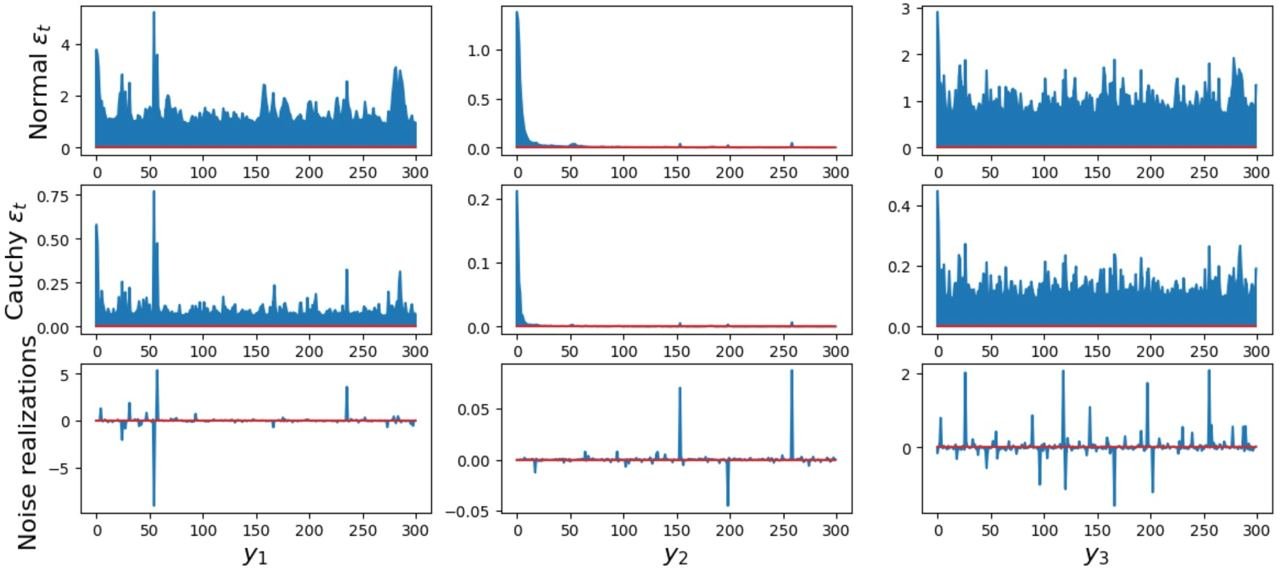
\includegraphics[width=0.9\columnwidth, height=\textheight,keepaspectratio]{figures/prm/abc_scales_evolution_cauchy.jpg}}
\label{fig:prm_abc_scales_evolution_cauchy}
\end{figure}

\section{Experiments conclusion}
It can be summarized that, within the framework of this chapter, the results of experiments showed the absolute superiority of ABC filters over the others in the conditions that the measurement model is misspecified, namely in conditions of ignorance of the noise of measurement distribution. It would be relevant to emphasize the stability of ABC filters again under different realizations of heavy-tailed noise, regardless of the choice of kernel.
